\documentclass[12pt]{article}
\usepackage{enumitem}
\usepackage[margin=1in]{geometry}
\usepackage{amsmath} 
\usepackage{amssymb}
\usepackage{graphicx}
\graphicspath{ {images/} }
\usepackage{titlesec}
\usepackage[utf8]{inputenc}
\usepackage[english]{babel}
\usepackage{blindtext}
 
\usepackage{multicol}


\title{Room Swapping Optimization}
\author{Lauren Leach, Ryan Sachs, Lisa Maszkiewicz}
\date{\today}

\begin{document}
 
\maketitle
 
\begin{multicols}{2}

\section{Introduction}

\subsection{Problem Statement and Goal}
\subsection{Current Roommate Swap Program}
\subsection{Expected Outcomes}

\section{Solution Overview}
\subsection{Preferences}
\subsection{Model}

\section{Preferences}
\subsection{Specific Preferences we considered}
\subsection{How specific preferences result in a weight}
\subsection{Ideas we kept, rejected, and that could be considered later}

\section{Model}
\subsection{Some Kind of Graph?}

\section{Integer Programming}
\subsection{TODO}

\end{multicols}

\section{Optimization Algorithm}

Up until now we've thought of our rooms as nodes in a graph. Now we'll look at the data as sets of potential occupants of the room. First, some terminology:\\

\noindent{Rooms $R$; \qquad with each $r\in\mathbb{R}$\qquad with capacity $c_r\in\mathbb{Z^+}$}\\
\noindent{Students $S$; \qquad with each $s\in\mathbb{S}$}\\ 

\noindent We're going to be doing most of our optimizing on variable x:\\

\begin{equation*}
\noindent{x_r^s \in \{0, 1\}\\} 
\end{equation*}

%{$r'$ is room \#\\

\noindent{$s$ is student \#\\
$r$ is old room \#}

\noindent{0 if they don't go to room, 1 if they do. }\\

What we're going to be maximizing, since this is an optimization problem, is W(R,S). As you recall each edge has a weight w(r,s), and W is the sum of all of the weights from each student wherever they end up. So our optimization equation is:\\

\begin{equation*}
\max\sum_{r\in{R}}\sum_{s\in{S(p)}}w(r,s)\cdot{x_s^r}\quad{s.t.}\\
\end{equation*}

With the constraints that each student gets assigned to a room and makes sure each only gets assigned to one room.

\begin{align*}
\forall{s}&\in{S}\sum_{r\in{R}}\sum_{s\in{S(p)}}x_s^r=1\\
\forall{r}&\in{R}\sum_{s\in{S(r)}}x_s^r=1
\end{align*}

Here we're going to put our example:\\

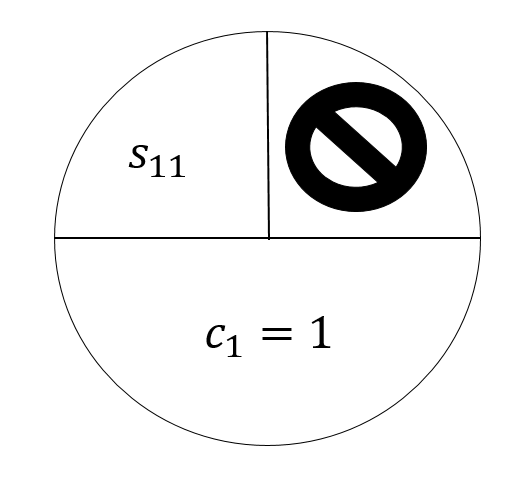
\includegraphics[scale=0.25]{c1} %\qquad \qquad
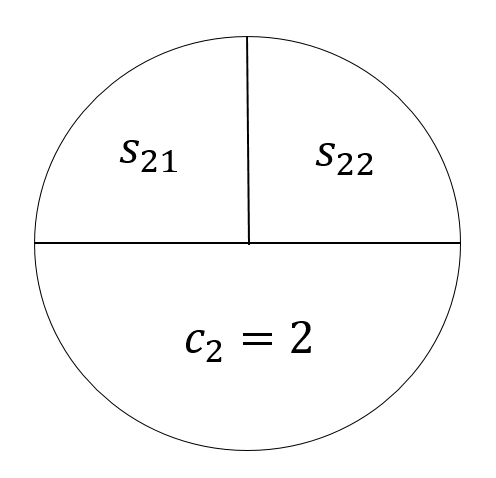
\includegraphics[scale=0.25]{c2} %\qquad \qquad
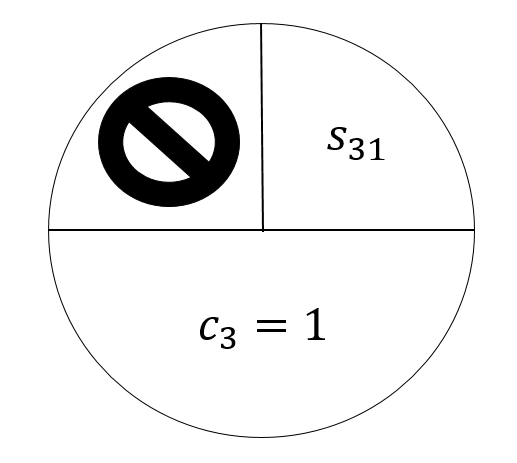
\includegraphics[scale=0.25]{c3}

\includegraphics[scale=1]{symbol}

%\{s_{11}, s_{21}, s_{22},s_{31}\}$
\begin{equation*}
\{\{s_{11}, s_{21}\}, \{s_{11},s_{22}\},\{s_{11},s_{31}\},  \{s_{21},s_{22}\}, \{s_{21},s_{31}\},  \{s_{22},s_{31}\} \}\implies x_r^s \in \{0, 1\}
\end{equation*}

\begin{align*}
x_2^1+x_1^2+x_4^2&=1\\
x_5^2+x_2^3&=1\\
\end{align*}

\begin{multicols}{2}

\section{Future Work- If we had more time}
Initially we struggled to determine what we should do to show results for our algorithm. We were originally thinking we would want to compare the same inputs on our system as theirs and see which was better. However, we got no information from Reslife throughout the semester so using results in our analysis at all wasn't going to happen. We had to choose a new way to validate our work.

\subsection{Testing Speed of Algorithm}
Our first attempt to try and  we might just run our own algorithm on 10 students, then 100, then 10,000 to see how the speed decreases with runs. But, we realized that wasn't really a useful metric to rate our algorithm by because not that many students enter the room swap. UMD has 4,000 students living on campus so it doesn't really reach that volume.

\subsection{Surveys}
During our presentation in class professor Hicks suggested that we could survey peoople to find out how they feel about their room situation.

\section{Works Cited}
"Introduction to Integer Programming - Integer Programming Models." The Lancet (2013). http://ocw.mit.edu. MIT OpenSourceWare, 14 Mar. 2013. PDF.

\end{multicols}
\end{document}